% Defino el tipo de documento.
\documentclass[a4paper,11pt]{article}

% Este paquete permite hacer encabezados y pies de p�gina como
% Los de las gu�as de D�az.
%\usepackage{fancyhdr}

% Este es para poder poner gr�ficos y diagramas.
\usepackage{graphicx}

% Este paquete est� por las dudas... Si algun archivo eps se vuelve
% rebelde y no sale donde uno quiere, hay que encajarle "\FloatBarrier" antes
% y despues y listo.
\usepackage{placeins}



% Toda la configuraci�n del documento.
%\input{preambulo.tex}


%\usepackage{grffile}
%\usepackage[dvips]{graphicx}


\hyphenation{}

\renewcommand{\sectionmark}[1]{\markboth{}{\thesection\ \ #1}}


\title{Evaluaci\'on Final de Simulaci\'on de Sistemas }

\author{45.288 Brasca, Juan Alejandro\\45.020 Stancato, Lucila\\45.002 Modernell, Dami\'an\\45.418 Negro, Conrado Luis}
\date{}

% Empieza el documento.
\begin{document}
\maketitle

%%%%%%%%%%%%%%%%%%%%%%%%%%%%%%%%%%%%%%%%%%%%%%%%%%%%%%%%%%%%%%%%%%%%%%%%%%%%%%%
\section*{a)   Modelar el intervalo de tiempo entre arribos, a partir de los datos medidos del archivo
$llegadasregistro$ y modelar el intervalo de tiempo de atenci\'on de la estaci\'on E3 con los
datos del archivo $e3registro$. Para ello hacer estad\'istica descriptiva, justificando el n\'umero
de intervalo de clases y realizar los test pertinentes.
}
%%%%%%%%%%%%%%%%%%%%%%%%%%%%%%%%%%%%%%%%%%%%%%%%%%%%%%%%%%%%%%%%%%%%%%%%%%%%%%%

%%%%%%%%%%%%%%%%%%%%%%%%%%%%%%%%%%%%%%%%%%%%%%%%%%%%%%%%%%%%%%%%%%%%%%%%%%%%%%%
\subsection*{Tiempo entre arribos al sistema}
%%%%%%%%%%%%%%%%%%%%%%%%%%%%%%%%%%%%%%%%%%%%%%%%%%%%%%%%%%%%%%%%%%%%%%%%%%%%%%%
Mediante mediciones del horario de arribo de clientes al sistema, computamos
los intervalos de tiempo entre arribos, y los representamos en el histograma
de la figura 1. Est\'a dividido en 7 intervalos de clase determinados a partir
de la f\'ormula de Sturgess que observamos en la ecuaci\'on 1.
\begin{equation} %equation 1
 k = 1 + 3.3 Log(n)
\end{equation}
donde $k$ es el n\'umero de intervalos y $n$ es el n\'umero de muestras.

\begin{figure} %figure 1
\begin{center}
\includegraphics[width=11cm]{histograma_llegadas}
\caption{Histograma de intervalos de tiempo entre arribos de clientes al sistema. Se puede observar que parece provenir de una variable aleatoria con distribuci\'on exponencial.}
\end{center}
\end{figure}

Como vemos en la figura 1, el tiempo entre llegadas de clientes parece ser una variable aleatoria
con distribuci\'on exponencial. Para determinar si esta suposici\'on es cierta, realizamos el test
de bondad de ajuste $\chi^2$. Las hip\'otesis del test son:

\begin{itemize}
 \item {$H_{0}$:} $\chi_{0}^2 < \chi_{n-1,\alpha}$ (Las llegadas de clientes al sistema est\'an exponencialmente distribuidas)
 \item {$H_{1}$:} $\chi_{0}^2 \ge \chi_{n-1,\alpha}$ (Las llegadas de clientes al sistema NO est\'an exponencialmente distribuidas)
\end{itemize}

A partir de las mediciones y de los valores esperados para cada intervalo de clase,
computamos el estad\'istico $\chi_{0}^2 = 10.709$. Como el valor
cr\'itico con un nivel de significaci\'on de 5\% y con 5 grados de libertad resulta 
$\chi_{0.05,5}^2 = 11.07$, rechazamos $H_1$ en favor de $H_0$.\\
Tambi\'en realizamos el test de Kolmogorov-Smirnov sobre las mediciones de los tiempos de arribos con las mismas hip\'otesis que el test $\chi^{2}$.
Obtenemos el estad\'istico para dichos datos $D =  0,1238$, con un valor cr\'itico para un nivel
de significaci\'on $\alpha = 5\% $, que es  $D_{5,0.05} = 0.4834$. Luego al ser $D < D_{t, \alpha }$,
se rechaza $H_1$ en favor de $H_0$.\\
Habiendo superado ambos tests, podemos suponer que los arribos de clientes al sistema est\'an
exponencialmente distribuidos , con una tasa media de $18.825$.

%%%%%%%%%%%%%%%%%%%%%%%%%%%%%%%%%%%%%%%%%%%%%%%%%%%%%%%%%%%%%%%%%%%%%%%%%%%%%%%
\subsubsection*{Tasa de servicio de la estaci\'on $E3$}
%%%%%%%%%%%%%%%%%%%%%%%%%%%%%%%%%%%%%%%%%%%%%%%%%%%%%%%%%%%%%%%%%%%%%%%%%%%%%%%
Analizamos los tiempos de servicio de la estaci\'on $E3$ medidos del sistema, y volcamos
los datos a un histograma (ver figura 2) con 8 intervalos de clase tambi\'en computados
a partir de la f\'ormula de Sturgess.

\begin{figure} %figure 2
\begin{center}
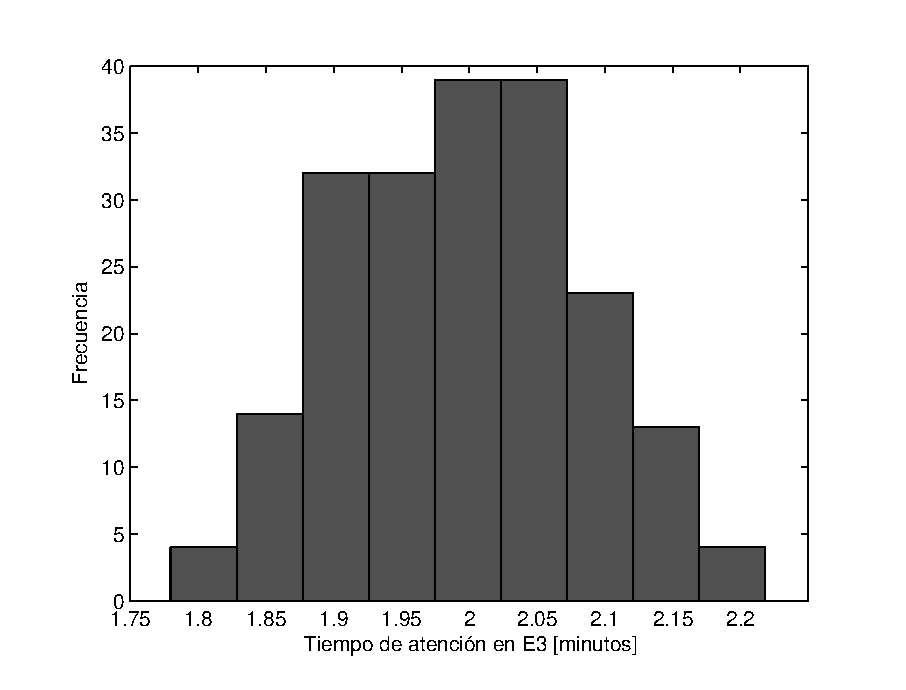
\includegraphics[width=11cm]{histograma_e3}
\caption{Histograma de la medici\'on de los tiempos de servicio del servidor $E3$. Observamos que los datos parecen provenir de una variable aleatoria con distribuci\'on normal.}
\end{center}
\end{figure}

En la figura 2, observamos que los datos parecen provenir de una variable aleatoria con distribuci\'on normal.
Para poder determinar si esto es cierto, realizamos el test estad\'istico $\chi^2$ con las siguientes hip\'otesis:

\begin{itemize}
 \item {$H_{0}$:} $\chi_{0}^2 < \chi_{n-1,\alpha}$ (El tiempo de servicio de la estaci\'on $E3$ es una variable aleatoria con distribuci\'on normal)
 \item {$H_{1}$:} $\chi_{0}^2 \ge \chi_{n-1,\alpha}$ (El tiempo de servicio de la estaci\'on $E3$ NO es una variable aleatoria con distribuci\'on normal)
\end{itemize}

Estimamos la media y la varianza de la distribuci\'on resultando:
\begin{itemize}
 \item {$\mu$ =} $1.995$
 \item {$\sigma^2$ =}  $0.008332$
\end{itemize}

El valor del estad\'istico resulta $\chi_{0}^2 = 4,7492$, y como el valor
cr\'itico es $\chi_{5,0.05}^2 = 11.07$ rechazamos $H_1$ en favor de $H_0$.\\

%%%%%%%%%%%%%%%%%%%%%%%%%%%%%%%%%%%%%%%%%%%%%%%%%%%%%%%%%%%%%%%%%%%%%%%%%%%%%%%
\section*{b) Indicar las variables de estado del sistema y el espacio de estados.}
%%%%%%%%%%%%%%%%%%%%%%%%%%%%%%%%%%%%%%%%%%%%%%%%%%%%%%%%%%%%%%%%%%%%%%%%%%%%%%%

Considerando el gr\'afico de la figura 3, definimos el espacio de estados S:\\

$ S = \{ ( x_R, x_{E_1}, x_{OFT}, x_{PSF}, x_{E_2}, x_{E_3}, x_{C_1}, x_{C_2}, x_{C_3},$ \\
     $y_R, y_{E_1}, y_{OFT}, y_{PSF}, y_{E_2}, y_{E_3}, y_{C_1}, y_{C_2}, y_{C_3} ) \/ $ \\
     $x_R, x_{E_1}, x_{OFT}, x_{PSF}, x_{E_2}, x_{E_3}, x_{C_1}, x_{C_2}, x_{C_3} = 1, 2, 3, ...$\\
     $\wedge y_R, y_{E_1}, y_{OFT}, y_{PSF}, y_{E_2}, y_{E_3}, y_{C_1}, y_{C_2}, y_{C_3} =  0, 1 \}$

Donde: \\
 $x_R$ es la longitud de la cola de recepci\'on.\\
$x_{E_1}$ es la longitud de la cola del servidor E1.\\
$x_{E_2}$ es la longitud del servidor E2.\\
$x_{E_3}$ es la longitud del servidor E3.\\
$ x_{OFT}$ es la longitud de la cola de oftalmolog\'ia.\\
$x_ {PSF}$ es la longitud de la cola del estudio Psico-F\'isico.\\
$x_{C_1}$ es la longitud de la cola de la caja C1.\\
$x_{C_2}$es la longitud de la cola de la caja C2.\\
$x_{C_3}$es la longitud de la cola de la caja C3.\\ \\
\noindent
$y_R$ Ocupac\'on de la recepci\'on.\\
$y_{E_1}$ Ocupaci\'on de la estaci\'on E1.\\
$y_{E_2}$ Ocupaci\'on de la  estaci\'on E2.\\
$y_{E_3}$ Ocupaci\'on de la  estaci\'on E3.\\
$y_{OFT}$ Ocupaci\'on del consultorio oftalmol\'ogico\\
$y_{PSF}$ Ocupaci\'on del consultorio Psico-Fisico.\\
$y_{C_1}$ Ocupaci\'on de la caja 1.\\
$y_{C_2}$ Ocupaci\'on de la caja 2.\\
$y_{C_3}$ Ocupaci\'on de la caja 3.\\

Sabiendo el valor de cada una de estas variables, se puede determinar el estado del
sistema completo.

\begin{figure} %figure 3
\begin{center}
\includegraphics[width=6cm]{automata}
\caption{Modelo del sistema de renovaci\'on del registro.}
	\end{center}
\end{figure}

%%%%%%%%%%%%%%%%%%%%%%%%%%%%%%%%%%%%%%%%%%%%%%%%%%%%%%%%%%%%%%%%%%%%%%%%%%%%%%%
\section*{c) Indicar los tipos de eventos y el espacio de eventos.}
%%%%%%%%%%%%%%%%%%%%%%%%%%%%%%%%%%%%%%%%%%%%%%%%%%%%%%%%%%%%%%%%%%%%%%%%%%%%%%%

El espacio de eventos $E$ del sistema lo definimos como:\\

$E = \{ A, D, r_{e1}, e1_{e3}, e3_{oft}, oft_{psf}, oft_{e2}, psf_{e2}, oft_{e1}, psf_{e1}, e2_{c1}, e2_{c2}, e2_{c3},  c1_{e2}, c2_{e2}, c3_{e3} \}$

Donde:\\
$A$ es la entrada de una persona a $R$.\\
$D$ es la partida de una persona del sistema (ya sea desde $R$, $E_1$ o $E_2$). \\
$r_{e1}$ es la partida de una persona desde $R$ hacia  $E_1$\\
$e1_{e3}$ es la partida de una parsona de $E_1$ hacia $E_3$ \\
$e3_{oft}$ es la partida de una persona de $E_3$ hacia $OFT$\\
$oft_{psf}$ es la partida de una persona de $OFT$ hacia $PSF$.\\
$oft_{e2}$, $psf_{e2}$ son las partidas de una persona desde $OFT$ o desde $PSF$ hacia $E_2$.\\
$oft_{e1}$, $psf_{e1}$ son las partidas desde $OFT$ o de $PSF$ hacia $E_1$\\
$e2_{c1}$, $e2_{c2}$ y $e2_{c3}$ son las partidas desde $E_2$ hacia $C_1$, $C_2$ y $C_3$.\\ 
$c1_{e2}$, $c2_{e2}$ y $c3_{e2}$ son las partidas desde $C_1$, $C_2$ y $C_3$ hacia $E_2$.\\

%%%%%%%%%%%%%%%%%%%%%%%%%%%%%%%%%%%%%%%%%%%%%%%%%%%%%%%%%%%%%%%%%%%%%%%%%%%%%%%
\section*{d)      Realizar una simulaci\'on indicando las condiciones iniciales, el tipo de generador usado y
la semilla. Mostrar las g\'aficas de las colas en cada estaci\'on.
}
%%%%%%%%%%%%%%%%%%%%%%%%%%%%%%%%%%%%%%%%%%%%%%%%%%%%%%%%%%%%%%%%%%%%%%%%%%%%%%%

Para generar n\'umeros pseudoaleatorios, usamos el generador de L'Ecuyer con semillas 50 y 23 (recordando
que lo importante es que las semillas no sean cero). El generador de L'Ecuyer genera una secuencia de n\'umeros
pseudoaleatorios con distribuci\'on uniforme entre 0 y 1. A partir de esa secuencia, generamos secuencias de n\'umeros pseudoaleatorios
con distribuci\'on exponencial. Para generar una secuencia de n\'umeros pseudoaleatorios con distribuci\'on normal usamos
el generador de Box-Muller (usando el generador de L'Ecuyer para generar la secuencia que tiene distribuci\'on uniforme).
Con estos generadores, podemos obtener realizaciones de las variables necesarias para simular el modelo.\\
Para hacer la simulaci\'on consideramos que el porcentaje de personas con m\'as de 70 a\~nos es de 7\%.   Esto hace
que la probabilidad de que un cliente haga el examen de aptitud psico�f\'isica pase de un 10\% (que renuevan el registro profesional) a un 17\%.
Consideramos tambi\'en que un 20\% de los clientes vienen solamente a buscar el instructivo para hacer el tr\'amite y se van,
y solamente el 80\% hace el tr\'amite de renovaci\'on. Adem\'as suponemos que un cliente tarda entre 0.5 y 2 minutos en llenar
el formulario que le entregan en la estaci\'on $E1$, y lo simulamos con una variable pseudo-aleatoria uniformemente distribuida.
Para las cajas $C_1$, $C_2$ y $C_3$, asumimos que los clientes se encolan en la caja que tenga menos personas, siempre optando primero por
$C_1$, luego por $C_2$ y como \'ultima opci\'on por $C_3$.

Con estas consideraciones, realizamos una simulaci\'on que termina a las 16:56 hs y atiende a 128 clientes. \\

En las figuras 4 a 12 podemos observar los estados de los servidores durante la simulaci\'on. Cuando el estado es 0,
la estaci\'on se encuentra desocupada, mientras que cuando vale 1 la estaci\'on se encuentra atendiendo a un cliente.

\begin{figure} %figure 4
\begin{center}
\includegraphics[width=12cm]{status_r}
\caption{Estado de la recepci\'on en funci\'on del tiempo. El primer cliente llega a las 8hs y las puertas se cierran a las 13hs.}
\end{center}
\end{figure}

\begin{figure} %figure 5
\begin{center}
\includegraphics[width=12cm]{status_e1}
\caption{Estado de la estaci\'on $E_1$ en funci\'on del tiempo. Se puede observar que aproximadamente a las 13hs, cuando no llegan m\'as clientes, la estaci\'on $E_1$ cesa sus actividades.}
\end{center}
\end{figure}

\begin{figure} %figure 6
\begin{center}
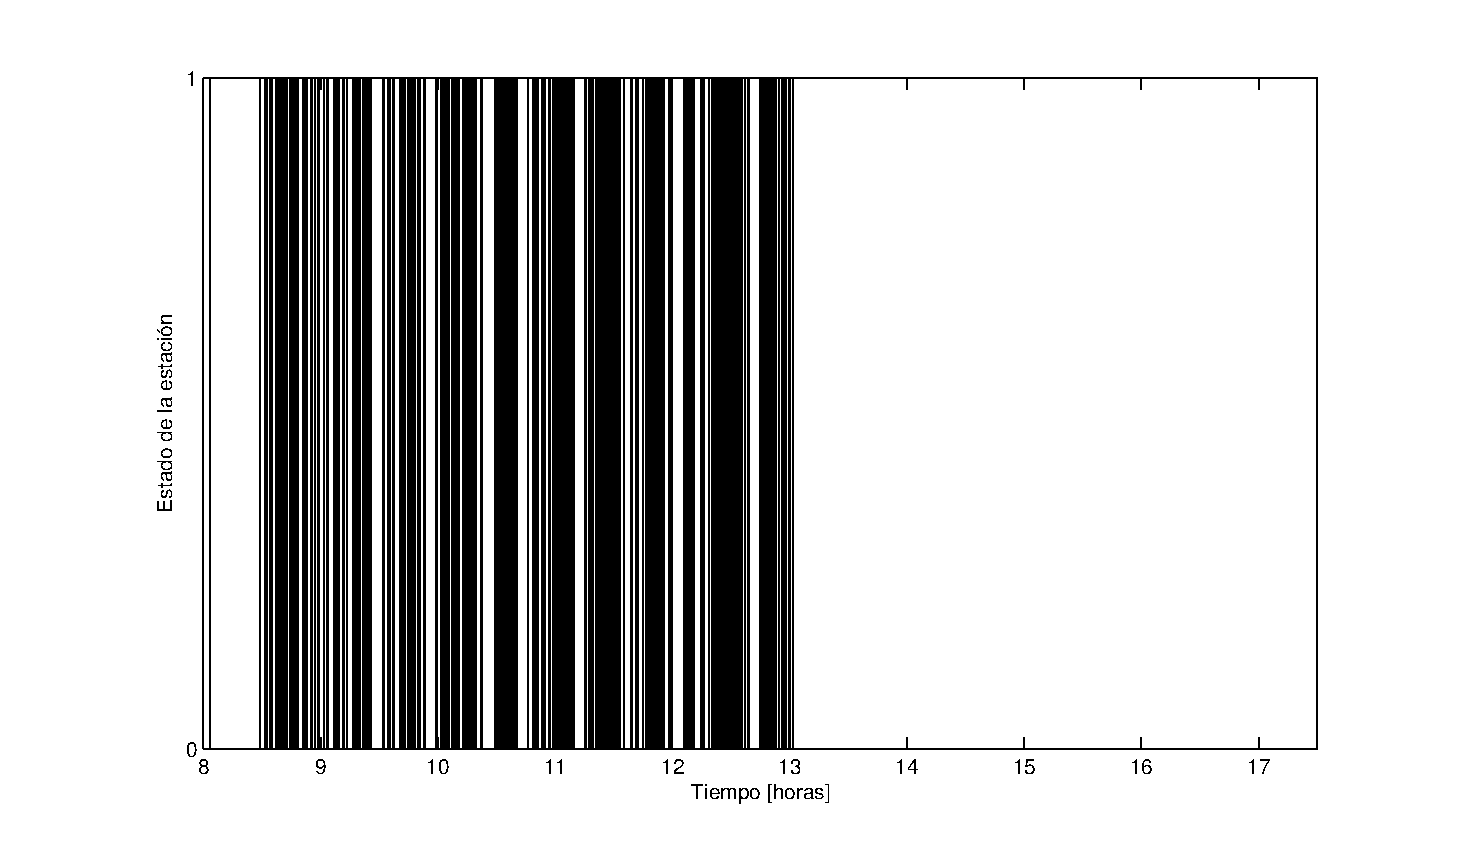
\includegraphics[width=12cm]{status_e3}
\caption{Estado de la estaci\'on $E_3$ en funci\'on del tiempo.}
\end{center}
\end{figure}

\begin{figure} %figure 7
\begin{center}
\includegraphics[width=12cm]{status_oft}
\caption{Estado del consultorio $OFT$ en funci\'on del tiempo.}
\end{center}
\end{figure}

\begin{figure} %figure 8
\begin{center}
\includegraphics[width=12cm]{status_psf}
\caption{Estado del consultorio $PSF$ en funci\'on del tiempo. Esta estaci\'on est\'a visiblemente menos ocupado que las dem\'as ya que s\'olo el 17\% de los clientes renuevan un registro profesional o son mayores de 70 a\~nos.}
\end{center}
\end{figure}

\begin{figure} %figure 9
\begin{center}
\includegraphics[width=12cm]{status_e2}
\caption{Estado de la estaci\'on $E_2$ en funci\'on del tiempo. Esta es la estaci\'on m\'as ocupada del sistema, ya que tiene un alto tiempo de atenci\'on en comparaci\'on con los otros, y adem\'as, recibe dos veces a cada cliente (cuando llegan de $OFT$ o $PSF$, y cuando llegan desde las cajas $C_1$, $C_2$ o $C_3$).}
\end{center}
\end{figure}

\begin{figure} %figure 10
\begin{center}
\includegraphics[width=12cm]{status_c1}
\caption{Estado de la caja $C_1$ en funci\'on del tiempo. Esta es la caja m\'as usada de las tres ya que los clientes la tienen como primer opci\'on a elegir cuando todas las cajas tienen una fila de la misma longitud. Si se encontrara ocupada, probar\'ian con la caja $C_2$, y luego con $C_3$.}
\end{center}
\end{figure}

\begin{figure} %figure 11
\begin{center}
\includegraphics[width=12cm]{status_c2}
\caption{Estado de la caja $C_2$ en funci\'on del tiempo. Esta es la segunda caja m\'as usada, ya que es elegida s\'olo si la caja $C_1$ tiene una fila m\'as larga que la caja $C_2$. }
\end{center}
\end{figure}

\begin{figure} %figure 12
\begin{center}
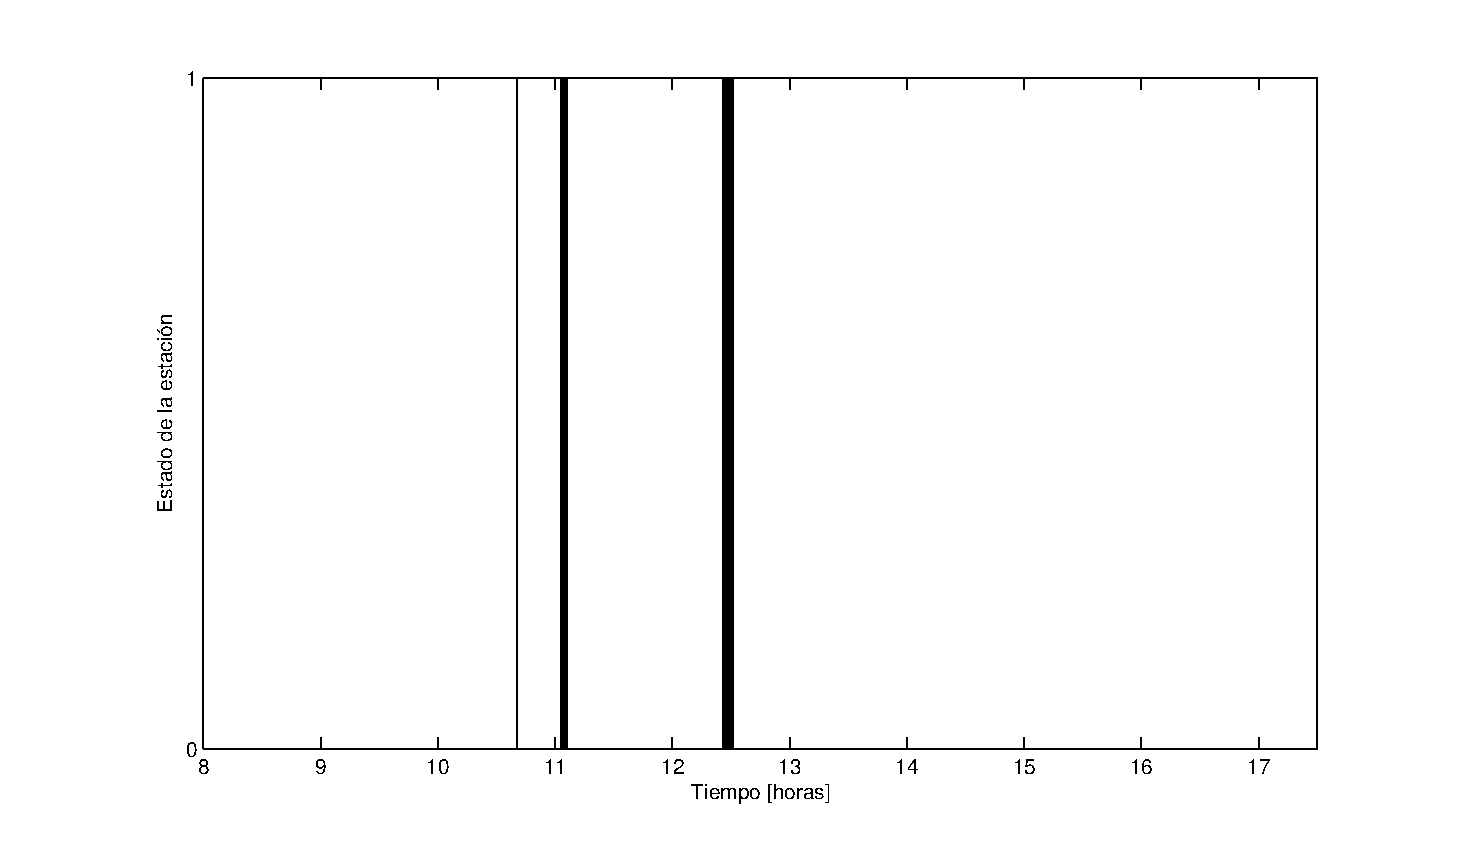
\includegraphics[width=12cm]{status_c3}
\caption{Estado de la caja $C_3$ en funci\'on del tiempo. Se puede observar el poco uso que los clientes hacen de esta caja, ya que $C_1$ y $C_2$ cumplen con casi todo el trabajo.}
\end{center}
\end{figure}

En las figuras 13 a 16 se puede observar la longitud de cada cola en funci\'on del tiempo. Como las estaciones
$E_1$, $PSF$, $C_1$, $C_2$ y $C_3$ nunca tienen clientes en sus colas, no los graficamos. $E_1$ no tiene clientes
en su cola porque el tiempo medio de atenci\'on es de  3 segundos, y los clientes llegan a un ritmo
menor desde la recepci\'on que atiende clientes con tiempo medio de entre 5 y 30 segundos. La estaci\'on $PSF$ nunca
tiene cola ya que recibe solo al $17\%$ de los clientes que ingresan al sistema, y tiene tiempo de atenderlos sin 
acumular clientes en la misma. Por \'ultimo, al tener tres cajas, la longitud de las colas esta dividida entre las
tres, y el tiempo de atenci\'on de cada caja es menor que el tiempo de arribo de clientes a este sector.

\begin{figure} %figure 13
\begin{center}
\includegraphics[width=12cm]{cola_r}
\caption{Cantidad de clientes en la cola de la recepci\'on en funci\'on del tiempo.}
\end{center}
\end{figure}

\begin{figure} %figure 14
\begin{center}
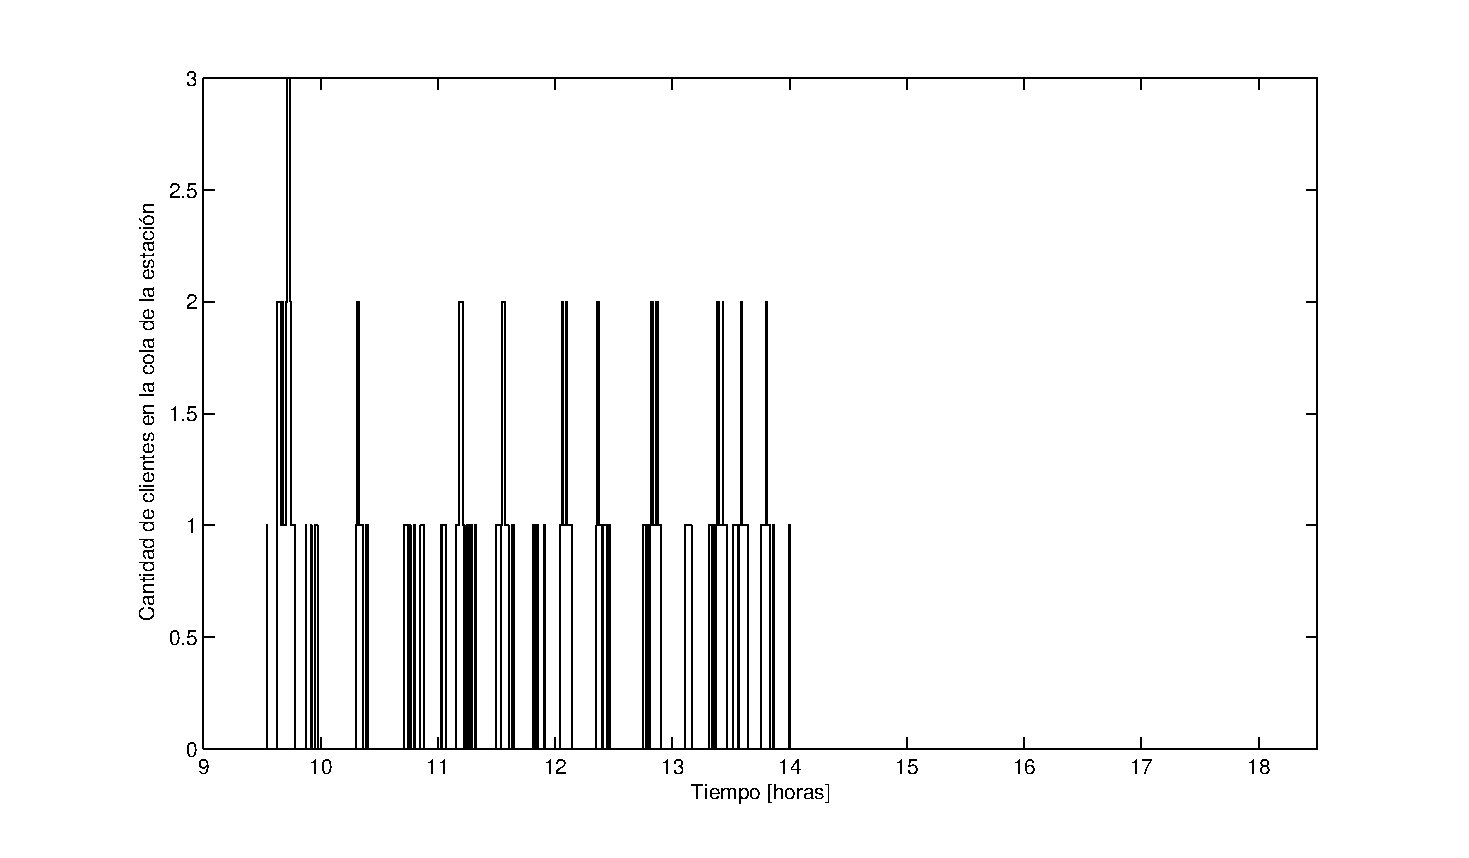
\includegraphics[width=12cm]{cola_e3}
\caption{Cantidad de clientes en la cola de la estaci\'on $E_3$ en funci\'on del tiempo.}
\end{center}
\end{figure}

\begin{figure} %figure 15
\begin{center}
\includegraphics[width=12cm]{cola_oft}
\caption{Cantidad de clientes en la cola del consultorio $OFT$ en funci\'on del tiempo.}
\end{center}
\end{figure}

\begin{figure} %figure 16
\begin{center}
\includegraphics[width=12cm]{cola_e2}
\caption{Cantidad de clientes en la cola de la estaci\'on $E_2$ en funci\'on del tiempo. Como esta es la estaci\'on m\'as ocupada del sistema, la cola que se genera hacia el final es la m\'as larga del sistema, llegando hasta 42 clientes.}
\end{center}
\end{figure}


%%%%%%%%%%%%%%%%%%%%%%%%%%%%%%%%%%%%%%%%%%%%%%%%%%%%%%%%%%%%%%%%%%%%%%%%%%%%%%%
\section*{e)     Realizar 10 simulaciones independientes. Hallar el tiempo medio por cliente en el sistema,
suponiendo que las tres cajas C1, C2 y C3 est\'an operativas mostrar los resultados convenien-
temente en una tabla. Computar con estos resulatados el estimador del tiempo medio por
cliente y su error.
}



Realizamos 10 simulaciones con diferentes semillas. En cada simulaci\'on se mide el tiempo medio  $\bar{t}$ de un cliente en el sistema,
la cantidad $N$ de clientes, y la hora $t_{final}$ a la que finaliza la simulaci\'on .  Los resultados se muestran en la tabla 1.


\begin{table}[!t]
\begin{center}
Tabla 1: Simulaciones con distintas semillas
\end{center}
\renewcommand{\arraystretch}{1.3}
%\caption{Simulaciones con distintas semillas}
\centering
\begin{tabular}{r r r r r }
\hline
\hline
Semilla 1 & Semilla 2 & $\bar{t}$ [hs] & $N$ & $t_{final}$ [hs]\\
\hline
50		&	23		&	1:45	&	128	&	16:56\\
150		&	263		&	1:50	& 	125	&	16:39\\
18		&	639		&	1:17	&	119 &	15:39\\
9018	&	78639	&	2:40	&	122 &	17:39\\
19018	&	278639	&	1:13	&	129 &	16:10\\
111		&	223		&	2:16	&	127 &	17:03\\
41114	&	82238	&	2:37	&	123 &	17:59\\
4199114	&	9		&	1:35	&	132 &	16:08\\
9		&	4199114	&	1:58	&	141 &	17:25\\
90		&	70		&	1:39	&	119 &	16:24\\

\hline
\hline
\end{tabular}
\end{table}

A partir de las simulaciones realizadas computamos la media muestral del tiempo medio de un cliente en el sistema, y obtenemos $\bar{t}=1:53$ hs,
con un desvio muestral de $\sigma = 30.3369$.  El error de la estimaci\'on lo calculamos haciendo $\sigma_t = \sigma/\sqrt(n)$, lo que resulta en 
$\sigma_t = 9.5934$ minutos, es decir, un error del 8.5\%.



%%%%%%%%%%%%%%%%%%%%%%%%%%%%%%%%%%%%%%%%%%%%%%%%%%%%%%%%%%%%%%%%%%%%%%%%%%%%%%%


\section*{f)    Si la probabilidad de que la caja C3 est\'e operativa es p, computar el tiempo medio por
cliente en el sistema en funci\'on de p. Graficar.
}

Dada $p$, la probabilidad de que la caja $C_3$ est\'e operativa, realizamos distintas simulaciones para estimar el tiempo 
medio de un cliente en el sistema.  Los resultados de las simulaciones se muestran en la figura 17.
  Vemos que si la probabilidad de que la caja $C_3$ est\'e abierta, es menor que 0.9, entonces el tiempo medio de un cliente
  en el sistema se incrementa en 22 minutos.  Si bien se ve en las secciones anteriores, que la caja 3 es la que menos se usa, 
  hay una diferencia entre tener un sistema con 2 cajas o tener un sistema con 3 cajas.

\begin{figure} %figure 17
\begin{center}
\includegraphics[width=12cm]{punto_f}
\caption{Tiempo medio de un cliente en el sistema, en funci\'on de la probabilidad $p$ de que la caja $C_3$ est\'e operativa.}
\end{center}
\end{figure}


\section*{g)   Computar la probabilidad de que el tiempo medio de espera en la cola de OFT sea mayor
a 5 minutos
}

Para computar la probabilidad de que el tiempo medio de espera en la cola OFT sea mayor a 5 minutos, almacenamos
 el tiempo de espera de cada cliente en la cola OFT. Luego contamos la cantidad de clientes que tienen un tiempo
 de espera mayor a 5 minutos, y lo dividimos por la cantidad de clientes que esperaron.  Con las condiciones iniciales
 de la secci\'on \emph{d}, obtenemos que 40 clientes esperaron m\'as de 5 minutos, sobre un total de 85. Lo que indica
 que la probabilidad de que el tiempo de espera sea mayor a 5 minutos es de 0.5294.


% La variable aleatoria $OFT$ tiene distribuci\'on exponencial con tiempo medio de 3.5 minutos. Para determinar la probabilidad de que el tiempo medio
% de espera sea mayor a 5 minutos la obtenemos a trav\'es de las ecuaciones XXXXXXXXXXX

% \begin{equation}
%  P( OFT > 5 ) = 1 - P( OFT \leq 5 )
% \end{equation}
% entonces:
% \begin{equation}
% P(OFT > 5 ) = 1 - ( 1 - e^{- \frac{1}{3.5}5} )
% \end{equation}
% Finalmente la probabilidad resulta:
% \begin{equation}
%  P( OFT > 5 ) = 0.2397
% \end{equation}


\begin{thebibliography}{1}
\bibitem{IEEhowto:kopka}
http://es.wikipedia.org/wiki/Regla\_de\_Sturgess

\bibitem{IEEhowto:kopka}
http://www.cyta.com.ar/biblioteca/bddoc/bdlibros/guia\_estadistica/modulo\_8.htm

\bibitem{IEEEhowto:kopka}
Diaz, Alejandro: Notas de Clase Curso 2009, Simulaci\'on por Eventos Discretos

\end{thebibliography}


\end{document}
